\documentclass[format=acmsmall, review=true, screen=true, anonymous=false]{acmart}

\usepackage{booktabs} % For formal tables
\usepackage{subfigure}
\usepackage{algorithmic}

\usepackage[ruled]{algorithm2e} % For algorithms
\renewcommand{\algorithmcfname}{ALGORITHM}
\SetAlFnt{\small}
\SetAlCapFnt{\small}
\SetAlCapNameFnt{\small}
\SetAlCapHSkip{0pt}
\IncMargin{-\parindent}


% Metadata Information
\acmJournal{TACO}
\acmVolume{9}
\acmNumber{4}
\acmArticle{39}
\acmYear{2010}
\acmMonth{3}
\copyrightyear{2009}
%\acmArticleSeq{9}

% Copyright
%\setcopyright{acmcopyright}
\setcopyright{acmlicensed}
%\setcopyright{rightsretained}
%\setcopyright{usgov}
%\setcopyright{usgovmixed}
%\setcopyright{cagov}
%\setcopyright{cagovmixed}

% DOI
\acmDOI{0000001.0000001}

% Paper history
\received{February 2007}
\received[revised]{March 2009}
\received[accepted]{June 2009}


% Document starts
\begin{document}
% Title portion. Note the short title for running heads
\title{SCP: Shared Cache Partitioning for High-performance GEMM}
\titlenote{New Paper, Not an Extension of a Conference Paper.}

\author{Xing Su}
%% \orcid{1234-5678-9012-3456}
\affiliation{%
  \institution{National University of Defense Technology}
  \streetaddress{Yanwachi Main Street 109}
  \city{Changsha}
  \state{Hunan}
  \postcode{410073}
  \country{China}}
\email{xingsu@nudt.edu.cn}
\author{Xiangke Liao}
\affiliation{%
  \institution{National University of Defense Technology}
  \streetaddress{Yanwachi Main Street 109}
  \city{Changsha}
  \state{Hunan}
  \postcode{410073}
  \country{China}
}
\affiliation{%
  \institution{National Laboratory for Parallel and Distributed Processing}
  \streetaddress{Yanwachi Main Street 109}
  \city{Changsha}
  \state{Hunan}
  \postcode{410073}
  \country{China}
}
\email{xkliao@nudt.edu.cn}
\author{Canqun Yang}
\affiliation{%
  \institution{National University of Defense Technology}
  \streetaddress{Yanwachi Main Street 109}
  \city{Changsha}
  \state{Hunan}
  \postcode{410073}
  \country{China}
}
\email{chan0345@tsinghua.edu.cn}
\author{Jingling Xue}
\affiliation{%
 \institution{University of New South Wales}
 \city{Sydney}
 \postcode{NSW 2052}
 \country{Australia}
 }
\email{jingling@cse.unsw.edu.au}

\begin{abstract}
  GEneral Matrix Multiply (GEMM) is the most fundamental
  computational kernel routine in the BLAS library.
  To achieve high performance, in-memory data must be
  prefetched into fast on-chip caches before they are used.
  Two techniques, software prefetching and data packing,
  have been used to effectively exploit the capability of
  on-chip lastly-recent-used (LRU) caches,
  which are popular in traditional high-performance
  processors used in high-end servers and supercomputers.
  However, the market has recently witnessed a
  new diversity in processor design, resulting in high-performance processors
  equipped with shared caches with non-LRU replacement policies.
  This poses a challenge to the development of
  high-performance GEMM in a multi-threaded context.
  As several threads try to load data into a shared cache simultaneously,
  inter-thread cache conflicts will increase significantly.
  We present a Shared Cache Partitioning (SCP) method to
  eliminate inter-thread cache conflicts in the GEMM routines,
  by partitioning a shared cache into physically disjoint
  sets and assigning different sets to different threads.
  We have implemented SCP in the OpenBLAS library and
  evaluated it on Phytium 2000+,
  a 64-core AArch64 processor with private LRU L1 caches
  and shared pseudo-random L2 caches (per four-core cluster).
  Our evaluation shows that SCP has effectively reduced the
  conflict misses in both L1 and L2 caches in a highly-optimized GEMM implementation,
  resulting in an improvement of its performance by $2.75\%$ -- $6.91\%$.
\end{abstract}


%
% The code below should be generated by the tool at
% http://dl.acm.org/ccs.cfm
% Please copy and paste the code instead of the example below.
%
\begin{CCSXML}
<ccs2012>
<concept>
<concept_id>10002950.10003714.10003715.10003719</concept_id>
<concept_desc>Mathematics of computing~Computations on matrices</concept_desc>
<concept_significance>500</concept_significance>
</concept>
<concept>
<concept_id>10010520.10010521.10010528.10010536</concept_id>
<concept_desc>Computer systems organization~Multicore architectures</concept_desc>
<concept_significance>500</concept_significance>
</concept>
</ccs2012>
\end{CCSXML}

\ccsdesc[500]{Mathematics of computing~Computations on matrices}
\ccsdesc[500]{Computer systems organization~Multicore architectures}

%
% End generated code
%

\keywords{GEMM, BLAS, Optimization, Linear Algebra, High Performance Computing}

\maketitle

% The default list of authors is too long for headers.
%% \renewcommand{\shortauthors}{G. Zhou et al.}

\section{Introduction}\label{sec:intro}
Dense linear algebra libraries are the most fundamental software in
scientific and engineering computing domains.
Basic Linear Algebra Subprograms (BLAS)~\cite{blas}  defines a collection
of APIs which act as standard building blocks for dense matrix operations.
BLAS routines are divided into 3 levels,
level-1 for vector-vector operations,
level-2 for matrix-vector operations,
and level-3 for matrix-matrix operations.
Processor vendors often provide BLAS implementations
that are highly optimized for their processors,
such as Intel MKL, AMD ACML and NVIDIA cuBLAS.
The HPC community has also contributed several high-quality
BLAS implementations, e.g., ATLAS~\cite{atlas},
GotoBLAS~\cite{gotoblas}, OpenBLAS~\cite{openblas},
and BLIS~\cite{blis,blisport}.

Among the three levels of BLAS routines, level-3 provides the most opportunities
for optimization because it has the highest computational complexity (of $O(n^3)$).
Among all the level-3 operations, GEneral Matrix Multiply (GEMM) is
of the most interest because the 
other level-3 operations can be defined
in terms of GEMM and some level-1 and level-2 operations~\cite{gemmbased1}.
In the past, much effort has been spent on optimizing GEMM for different
architectures~\cite{Liu2012,Wang2015,Volkov:2008,Cui11,blispar}.
%% both in general algorithm and in architecture specific ways.

%% GEMM performs a matrix-multiply-accumulate operation.
An optimized GEMM implementation consists of two components,
(1) a highly optimized kernel routine to accomplish its
computation, and
(2) an overall strategy to partition the workload into small tasks
and schedule these tasks to be executed effectively on the target processor.
The kernel routine is a serial program performing matrix-multiply-accumulate
on matrices from a single task.
The overall strategy partitions the workload by tiling 
the underlying loop nest
and determines a task schedule by choosing a specific traversal order
in the loop nest's iteration space.
In a multi-threaded context, different tasks (loop tiles) are assigned to
different threads to parallelize the whole operation.
The main objective of GEMM optimization is to
maximize the floating-point
operation throughput, measured by FLoating-point Operations Per Second ($flops$).
For the serial kernel routine, the optimization applies
instruction scheduling to improve instruction throughput.
For the workload partitioning, the optimization 
reorganizes memory accesses to reduce long memory latencies for
the kernel.
In this paper, we focus on optimizing the memory accesses for GEMM.

Two techniques, software prefetching and data packing,
have been widely used in GEMM implementations to speed up memory accesses.
Software prefetch instructions are utilized
to load data into cache before they are used, in 
order to ensure that memory accesses will not incur
long latencies and floating-point instructions
can execute at peak throughput.
To better exploit the capability of on-chip caches,
matrices are blocked and then packed into continuous memory buffers
that can fit into the caches under consideration
before the kernel routine is called.
Because GEMM is a computational intensive operation whose
arithmetic complexity is $O(n^3)$ and memory complexity is $O(n^2)$,
the overhead caused by data packing is negligible when
the input matrices are large~\cite{gotogemm}.


However, software prefetching and data packing cannot be effectively
applied to architectures with non-LRU shared caches.
In traditional high-performance processors, e.g., the Intel Xeon series,
both L1 and L2 caches are private to processor cores
and LRU replacement policy is adopted.
Without considering the last level cache (LLC),
the threads running on different cores prefetch their data into
different caches, and private data of different threads
cannot cause conflict cache misses.
This is no longer the case if caches are shared by several processor cores.
In this case, a cache line prefetched by one thread
may be evicted before its lifetime ends because another thread prefetches
another cache line into the same cache set.
A simple-minded solution would be to reduce 
the size of a packed matrix
so that the data used by several threads can simultaneously reside in a shared cache.
Due to the nature of set-associative caches,
this solution cannot completely eliminate inter-thread cache conflicts,
especially if the shared cache has a non-LRU replacement policy.
Our evaluation shows that inter-thread cache conflicts
in non-LRU shared caches
can heavily hurt GEMM performance,
even with packed matrices reduced to fit into the cache.

Following the trend in recent decades, modern architecture design
is introducing more and more cores on a single processor chip.
To reduce cost of on-chip cache memories and coherence networks,
shared caches may become common in future many-core processors.
In addition, non-LRU replacement policies, for example, pseudo-random,
may also be used to further reduce the cache design complexity.
Indeed, some high-performance processors based on the
ARM technology, e.g., the Phytium processor series~\cite{phytium},
%% I'm sure they have shared L2 caches,
%% but have not found any technical specification about the replacement policy
%% XGene from AppliedMicro~\cite{xgene},
%% ThunderX from Cavium~\cite{thunderx}
have already adopted this design. 
As a result, developing a better solution to reduce
the inter-thread cache conflicts 
for non-LRU shared caches is important.

In this paper, we present a Shared Cache Partitioning (SCP) method
to reduce inter-thread cache conflicts on architectures with non-LRU share caches.
The key idea is to partition a
share cache into physically disjoint sets
and assign different sets to different threads. This can be achieved by
exploiting the memory mapping mechanism of set-associative caches.

To the best of our knowledge, SCP represents
the first work addressing
the inter-thread cache conflicts problem on
architectures with non-LRU share caches.

The main contributions of this paper are as follows:
\begin{itemize}
\item We present a quantitative analysis of the negative effect of inter-thread cache
  conflicts on GEMM performance.
\item We propose SCP, a method for solving the inter-thread cache conflicts
  problem on architectures with non-LRU shared caches.
\item We have implemented SCP in the OpenBLAS library and evaluated it on Phytium 2000+,
  an emerging high-performance processor based on ARM's AArch64 architecture.
  Phytium 2000+ has 64 cores, private LRU L1 caches
  and pseudo-random shared L2 caches.
  Our evaluation shows that SCP can improve the GEMM performance consistently
  under various parallelism configurations, by $2.75\%$--$6.91\%$.
\end{itemize}


The rest of the paper is organized as follows.
Section~\ref{sec:background} gives some background on GEMM and discusses
the cache conflicts incurred.
Section~\ref{sec:scp} introduces the SCP method.
Section~\ref{sec:evaluation} presents and
analyzes our experimental results.
Section~\ref{sec:related} reviews the related work.
Finally, Section~\ref{sec:conclusion} concludes.


\section{Background}\label{sec:background}

\subsection{The Memory Hierarchy Review}\label{subsec:hierarchy}

Modern architectures take advantage of fast on-chip caches
to overcome the ``memory wall''.
As a compromise between direct mapped caches
and full-associative caches,
set-associative caches have been the dominant choice for real-world architectures.
To understand how cache sharing causes
inter-thread cache conflicts
and hurts GEMM performance, we review some details
about the working mechanism of set-associative caches and
the memory hierarchy of modern processors.

A set-associative cache can be defined by a 4-tuple $(c, l, n, nt)$,
where $c$ is the cache capacity, $l$ is the cache line size,
$n$ is the number of ways-of-associativity,
and $nt$ indicates the number of cores sharing the cache.
The whole cache memory is divided into $ns=c/l/n$ sets,
identified by indices in $\mathcal{S} = [0, ns)$,
with each set containing $n$ cache lines.
Generally, $ns$ is a power-of-two.
An indexing function $\varphi: \mathcal{A} \mapsto \mathcal{S}$ is responsible for
mapping the addresses in the address space $\mathcal{A}$
(either virtual or physical) to the cache sets in
$\mathcal{S}$.
The data at $addr \in \mathcal{A}$ must be fetched
into the cache set $\varphi(addr) \in \mathcal{S}$ if requested.
A classic implementation of the indexing function is shown below,
%% $\varphi(addr) = (addr \gg \log_2(l)) ~\&~ (ns-1)$,
with $\gg$ and $\&$ representing logical-shift-right and bitwise-and operations, respectively:
\begin{equation*}
  \varphi(addr) = (addr \gg \log_2(l)) ~\&~ (ns-1)
  \label{eq:phi}
\end{equation*}
which represents an extraction of the $\log_2(ns)$ bits starting from the $\log_2(l)$-th
position in $addr$'s binary form.
It is easy to prove that any continuous memory block
that is no larger than $c/n$
cannot conflict with itself.
We therefore define a quantity, \emph{way-capacity}, denoted as $wc=c/n$,
to represent this size bound for conflict-free memory blocks.

The main memory, $NL$ levels of caches, and $NT$ processor cores
form a memory hierarchy are generally organized in terms
of an $NL+2$ level regular tree structure.
The processor cores at level $0$ are leaves,
the caches at levels $1$ -- $NL$ are intermediate nodes,
and the main memory at level $NL+1$ is the tree root.
Any node in the memory hierarchy can be identified by
its layer and its unique index at the layer $(layer, index)$.
The number of nodes at layer $l$ is $NT / nt_l$.

Throughout this paper, our example platform will be
a four-core processor with
$NL=2$ levels of caches.
Figure~\ref{fig:hierarchy} shows its memory hierarchy 
and Table~\ref{tab:cluster} lists its
architectural parameters. 
Each core has 32 128-bit (16B) vector registers,
each capable of storing two double-precision floating-point numbers.
For convenience, a processor core at level 0
is represented by its registers, which can be viewed as a special
level-0 cache $L0 = (512B, 16B, 32, 1)$ with a programmable replacement policy.

\begin{figure}
  \centering
  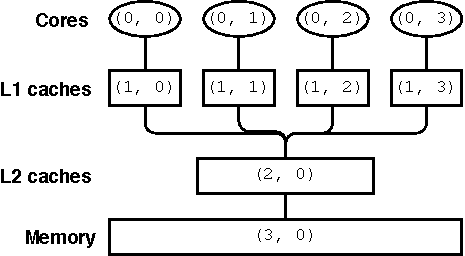
\includegraphics[width=.65\textwidth]{figures/cluster-new}
  \caption{Memory hierarchy of the four-core processor
    (nodes labeled with $(layer,index)$)}
  \label{fig:hierarchy}
\end{figure}

\begin{table}
  \centering
  \caption{Architectural parameters of the four-core processor}
  %% (see Section~\ref{subsec:hierarchy} for meanings of symbols in the header row)
  \label{tab:cluster}
  \begin{tabular}{lccccccl}
    \toprule
    Type & $c$ & $n$ & $l$ & $nt$ & $ns$ & $wc$ & Policy \\
    \midrule
    L0 Registers  & 512B & 32 & 16B & 1 & 1 & 16B & Programmable \\
    L1 Data    & 32KB & 2  & 64B & 1 & 256 & 16KB & LRU \\
    L2 Unified & 2MB  & 16 & 64B & 4 & 2048 & 128KB & Pseudo-Random \\
    \bottomrule
  \end{tabular}
\end{table}

\subsection{Structure of GEMM}\label{subsec:gemm}

GEMM performs a matrix-multiply-accumulate operation $C = \beta C + \alpha A B$,
where $A, B$ and $C$ are matrices of sizes
$M \times K$, $K \times N$ and $M \times N$, respectively,
and $\alpha$, $\beta$ are scalars.
While this operation is algorithmically simple,
so that a 3-deep loop nest suffices to accomplish it,
a high-performance implementation can be quite
sophisticated due to the presence of multi-level memory
hierarchies on modern processors.
Figure~\ref{fig:gemm} shows the structure of GEMM from
the OpenBLAS library~\cite{openblas}.
Each loop (in the original 3-deep loop nest) is tiled,
resulting in a total of six loops (referred to as layers 1 -- 6).
%% Loop tiling, together with data packing and prefetching,
%% serves to improve data locality and overlap computation
%% and memory access effectively.

\begin{figure*}[t]
  \centering
  \includegraphics[width=\textwidth]{figures/gemm}
  \caption{Structure of blocked GEMM}
  \label{fig:gemm}
\end{figure*}

In this blocked algorithm, the $jj$, $kk$ and $ii$ loops
along the $N$, $K$ and $M$ matrix dimensions are
tiled by sizes $N_c$, $K_c$ and $M_c$ at layers 1, 2 and 3, respectively.
At layers 4 and 5, the $j$ and $i$ loops along the $N$ and $M$ dimensions
are further tiled by sizes $N_r$ and $M_r$, respectively.
As a result, the innermost loop at layer 6 goes over the $K$
dimension for a total of $K_c$ times,
with each iteration performing a rank-1 update on
the $M_r \times N_r$ sub-matrix of $C$, as shown at layer 7.
In OpenBLAS, matrix $C$ is scaled by $\beta$ before the loops,
so the multiply-accumulate operation at layer 7 does not have to scale $C$ again.
Tiling factors $N_c$, $K_c$, $M_c$, $N_r$ and $M_r$ are carefully selected so that
matrices at each level fit into a certain level in the memory hierarchy, with the following
constraints:
\begin{eqnarray}
  es (M_r + N_r + M_r N_r) & \le & c_{0} \label{eq:constraints.reg}\\
  nt_{1} \cdot es (N_r K_c + 2 M_r K_c) & \le & c_{1} \label{eq:constraints.l1}\\
  nt_{2} \cdot es (M_c K_c + 2 N_r K_c) & \le & c_{2} \label{eq:constraints.l2}\\
  es (N_c K_c + nt_{3} \cdot M_c K_c)   & \le & c_{3} \label{eq:constraints.l3}
\end{eqnarray}
where $es$ denotes the size of a matrix element,
e.g., 8B for a double-precision floating-point number
and $c_l$ ($0\leqslant l \leqslant 3$) denotes the capacity of the register file or cache at level $l$.
By (\ref{eq:constraints.reg}), $M_r$ and $N_r$ are so
constrained that $M_r$ elements from $A$,
$N_r$ elements from $B$ and $M_r \times N_r$ elements from $C$ can
fit into the registers (the pseudo level-0 cache).
By (\ref{eq:constraints.l1}), $K_c$ is so constrained that $B_4$ ($N_r \times K_c$),
$A_4$ ($M_r \times K_c$), and $A_4$'s counterpart in the next iteration
at layer 5 fit into the L1 cache.
By (\ref{eq:constraints.l2}), $M_c$ is so constrained that $A_3$ ($M_c \times K_c$),
$B_3$ ($N_r \times K_c$), and $B_3$'s counterpart in the next iteration
at layer 4 fit into the L2 cache.
Finally, by (\ref{eq:constraints.l3}), $N_c$ is so constrained that 
$B_2$ ($K_c \times N_c$) and $A_2$ ($M_c \times K_c$) fit into the L3 cache (if it exists).
Larger matrices at higher layers 1 -- 3 always reside in main memory.

\begin{comment}
Table~\ref{tab:factors} shows the procedure choosing various tiling factors.
In each row, one or more tiling factors (column 1) is determined
by a size constraint (column 3) related to a certain level
in the memory hierarchy (column 2).
\begin{table}
  \centering
  \caption{Procedure of choosing tiling factors}
  \label{tab:factors}
  \begin{tabular}{cccl}
    \toprule
    factor & memory & constraint \\
    \midrule
    $M_r$, $N_r$ & registers & $M_r + N_r + M_r N_r \le Regs$ \\
    $K_c$        & L1 cache  & $N_r K_c + 2 M_r K_c \le L1$ \\
    $M_c$        & L2 cache  & $M_c K_c + 2 N_r K_c \le L2$ \\
    $N_c$        & L3 cache  & $N_c K_c + M_c K_c \le L3$ \\
    \bottomrule
  \end{tabular}
\end{table}
\end{comment}

Goto~\cite{gotogemm} factors out the innermost three loops at layers 4 -- 6 for
computing $C_2\ = C_2 + \alpha A_2 B_2$ as an architecture-dependent kernel,
known as  GEBP (GEneral multiply of a Block of $A$ and a Panel of $B$).
It is worthy noting that before GEBP is called (at layer 3),
$A_1[ii:ii+M_c-1][:]$ and $B_1$ are packed into $A_2$ and $B_2$
in a special continuous layout,
so consecutive memory access is ensured within the GEBP kernel.
GotoBLAS~\cite{gotoblas}, and its successor, OpenBLAS~\cite{openblas},
implement GEMM programs based on this factorization,
with GEBP highly optimized for the target processor.

As stated in Section~\ref{sec:intro}, a GEMM implementation
is made up by a kernel routine and an overall workload-partitioning strategy.
In Figure~\ref{fig:gemm}, GEBP serves as the kernel routine,
and the workload-partitioning strategy is defined by the three outer loops at layers 1 -- 3.
Developers can decide how to partition the workload by choosing
tile factors $M_c$, $N_c$ and $K_c$,
and how to schedule the GEBP tasks by interchanging loop orders at layers 1 - 3.
Either the $jj$ loop at layer 1 or the $ii$ loop at layer 3, or both,
can be parallelized in a multi-threaded context.
Specifically, the implementation in Figure~\ref{fig:gemm}
chooses an $jj\textrm{-}kk\textrm{-}ii$ loop order
and parallelizes the $ii$ loop at layer 3.
Different threads work on different portions of $A_1$
but share the same $B_1$.

As a result, there are multiple $A_2$ instances (one per thread)
and a single $B_2$ instance (shared by all threads).
To understand how the $ii$ loop at layer 3 is parallelized on the four-core processor, 
Figure~\ref{fig:workload} shows the data accessing patterns
for a single thread $T_1$.
While all the color shaded submatrices are accessed by $T_1$,
only the submatrices highlighted by the z-curves
(a subset of color shaded ones) are packed by $T_1$.
In other words, each thread packs its own $A_2$ instance but all the threads pack collaboratively the unique $B_2$ instance.
%% We will use the OpenBLAS GEMM implementation in Figure~\ref{fig:gemm}
%% in discussion and evaluation throughout the paper.

\begin{figure}[t]
  \centering
  \includegraphics[width=.5\textwidth]{figures/workload}
  \caption{GEMM parallelization with four threads and data accessing patterns of thread $T_1$}
  \label{fig:workload}
\end{figure}

\subsection{Cache Conflicts in GEMM}\label{subsec:cache-conflicts}

For set-associative caches, cache misses can be categorized
into capacity and conflict misses.
While (\ref{eq:constraints.reg}) -- (\ref{eq:constraints.l3})
aim to avoid capacity misses,
conflict misses cannot be eliminated completely.
%% We use the term ``cache conflict'' to represent conflict miss events.

In Figure~\ref{fig:gemm}, the packed matrix $A_2$
will be read $N_c/N_r$ times within a single GEBP execution,
and is expected to reside in the 
L2 cache during all the $N_c/N_r$ iterations at layer 4.
The packed matrix $B_4$ is similar in that it is expected to
reside in the L1 cache during all the
$M_c/M_r$ iterations at layer~5.
In general, even with carefully selected tile factors,
some matrix elements can still be evicted.
For example, some data structures other than the packed matrices
or program code (in case of a unified cache) may be fetched into the
cache set where these matrix elements reside in.
Such cache conflicts are known as
\emph{intra-thread cache conflicts}
because they occur within the execution of a single thread.
To deal with intra-thread cache conflicts,
the GEBP kernel repeatedly prefetches data from $A_4$ and $B_4$ to the L1 cache
during every iteration at layer 6 before it actually reads them just in case that
the data may have been evicted accidentally from the L1 cache.
As GEBP accesses the matrix data much more frequently than other
data structures, this repeated prefetching strategy
can reduce the penalty caused by intra-thread cache conflicts.

In contrary to intra-thread cache conflicts,
there exists another kind of cache conflicts, called
\emph{inter-thread cache conflicts}, on architectures with shared caches.
Suppose two working threads, $T_0$ and $T_1$, are running independently
on the four-core processor in Figure~\ref{fig:hierarchy}
to accomplish a GEMM operation.
At time $t_s$, $T_0$ prefetches some data at address $addr_0$
to the cache set $\varphi_2(addr_0)$ in the shared L2 cache.
The data will be actually read at time $t_e$.
Then at some time $t_m$ ($t_s < t_m < t_e$),
$T_1$ prefetches data at address $addr_1$ to the L2 cache.
If $\varphi_2(addr_1)=\varphi_2(addr_0)$, then the
data at $addr_1$ and $addr_0$ will be fetched into the same cache set.
As the shared L2 cache has a non-LRU policy,
the data at $addr_0$ may suffer an eviction before it is actually read,
i.e., a conflict miss occurs.

In GEMM, every cache is utilized aggressively
so that almost all its cache space is expected to be occupied by packed matrices.
Prefetch instructions from different threads are executed repeatedly,
interleaved in an unpredictable manner.
So inter-thread cache conflicts described above
can occur frequently for shared non-LRU caches,
thus making the technique dealing with intra-thread cache conflicts ineffective.
The situation worsens with more threads sharing the same cache.



\section{SCP: The Shared Cache Partitioning Method}\label{sec:scp}

This section demonstrates the SCP method to handle inter-thread cache conflicts.
The basic idea is that inter-thread cache conflicts can be eliminated
if packed matrices used by different threads are fetched to different cache sets.
In Section~\ref{subsec:example}, we demonstrate SCP by an example.
Then a formal description is given in Section~\ref{subsec:formal}.

\subsection{Example}\label{subsec:example}

Suppose we are implementing a double precision GEMM (DGEMM) on
the 4-core processor, i.e., $es=8B$.
We now determine the tiling factors used in DGEMM following the procedure described
by constraints (\ref{eq:constraints.reg})--(\ref{eq:constraints.l3}).
Various configurations for ($M_r$, $N_r$) can satisfy (\ref{eq:constraints.reg}),
e.g., $(4,8)$, $(8,4)$, $(6,8)$, and $(8,6)$. 
It takes careful consideration to determine which one is the best,
and a tuning process may be needed.
After tuning we obtain the best values $M_r = 4$ and $N_r = 8$.
By (\ref{eq:constraints.l1}),
$K_c \le \lfloor c_{L1}/es/nt_{L1}/(N_r + 2 M_r) \rfloor = \lfloor 32KB/8B/1/16 \rfloor = 256$.
Here we choose $K_c=256$.
By (\ref{eq:constraints.l2}),
$M_c \le \lfloor (c_{L2}/es/nt_{L2} - 2 N_r K_c )/ K_c \rfloor =
\lfloor (2MB/8B/4 - 2*8*256)/256 \rfloor = 240$.
To leave space for other data structures, as well as the program code,
it is reasonable to shrink $M_c$ to a slightly smaller value,
e.g., $192$, $208$ and $224$ are all proper candidates for $M_c$.
Similar to $M_r$ and $N_r$, a tuning process may be needed to
find the best value for $M_c$.
Here we choose $M_c = 192$.
As there is no L3 cache, (\ref{eq:constraints.l3}) can be ignored
and $N_c$ can be given a large value.
Here we choose $N_c = 1024NT = 4096$.
With tiling factors determined, the sizes of packed matrices
can be calculated. Table.~\ref{tab:msizes} list the sizes of
various packed matrices.

\begin{table}
  \centering
  \caption{Sizes of packed matrices in DGEMM ($es = 8B$)}
  \label{tab:msizes}
  \begin{tabular}{cl|cl}
    \toprule
    matrix & size & matrix & size \\
    \midrule
    %% $A_2$, $A_3$ & $es M_c K_c = 384KB$ & $B_2$ & $es N_c K_c = 8MB$ \\
    %% $A_4$ & $es M_r K_c = 8KB$   & $B_3$, $B_4$ & $es N_r K_c = 16KB$ \\
    $A_2$ & $es M_c K_c = 384KB$ & $B_2$ & $es N_c K_c = 8MB$ \\
    $A_3$ & $es M_c K_c = 384KB$ & $B_3$ & $es N_r K_c = 16KB$ \\
    $A_4$ & $es M_r K_c = 8KB$   & $B_4$ & $es N_r K_c = 16KB$ \\
    \bottomrule
  \end{tabular}
\end{table}

\begin{figure}
  \centering
  \subfigure[Way-partitioning]{
    \label{fig:partition.conventional}
    \includegraphics[width=.4\textwidth]{figures/wpart}
  }
  \subfigure[Set-partitioning]{
    \label{fig:partition.segmented}
    \includegraphics[width=.4\textwidth]{figures/spart}
  }
  \caption{Partition styles of the shared L2 cache (n=16, ns=2048)}
  \label{fig:partition}
\end{figure}

Each $A_2$ is packed into a single continuous buffer.
Figure.~\ref{fig:partition.conventional} shows how the
$A_2$ instances of 4 threads are distributed in the shared 16-way L2 cache.
We see that every cache set $s \in [0,2048)$ contains
data from all 4 $A_2$ instances,
potentially leading to inter-thread cache conflicts.
What if the $A_2$ matrices are distributed in the way shown in
Figure.~\ref{fig:partition.segmented}?
$A_2$ of different threads live in strictly disjoint cache sets,
and inter-thread cache conflicts caused by $A_2$ are eliminated completely!

Figure.~\ref{fig:partition.conventional} and Figure.~\ref{fig:partition.segmented}
essentially represent two different partitioning styles of the shared cache,
referred to as way-partitioning and set-partitioning, respectively.
To guarantee the data layout in set-partitioning,
$A_2$ cannot be stored in a single continuous buffer any more.
Instead, $A_2$ is distributed to 12 continuous memory segments, each of size $32KB$.
The distance from one segment to the next is equal to $wc_2=128KB$.
%% There is no memory fragment because the segment size is a multiple of
%% size of $A_4$ (8KB).
%% FIXME put this to the end of this section
While the set-partitioning of shared caches avoids inter-thread cache conflicts,
it introduces some complexity to GEMM implementation
because the GEBP kernel and the matrix packing routines
now must work with segmented memory buffers instead of continuous ones.

How about $B_2$, the other packed matrix use in GEBP?
Unlike $A_2$, which is thread private,
$B_2$ is shared among all threads and
the packing of $B_2$ is done collaboratively by all threads.
We have two choices, privatize $B_2$ and apply the set-partitioning method,
or fall back to conventional way-partitioning for $B_2$.
$B_2$ can be made thread private if every thread makes
its own pack of the whole $B_1$ matrix.
The first choice achieves a full per-thread data isolation
at the expense of redundant packing overhead.
The second choice avoids the extra overhead in both time and space
but risks inter-thread conflicts caused by the shared $B_2$ matrix.
The two choices are evaluated and compared in Section~\ref{sec:evaluation}.

\subsection{Formal Description}\label{subsec:formal}
Given tiling factors $M_r$, $N_r$, $K_c$, $M_c$, $N_c$,
and architectural details of the memory hierarchy,
The SCP method systematically determines the
the memory layout for packed matrices $A_2$ and $B_2$ used in GEMM.
Memory layout of other packed matrices on lower layers are
determined by $A_2$ and $B_2$.
We assume that the share matrix $B_2$ is packed
in conventional way-partitioning style.
If desired, $B_2$ can be privatized and handled in the same way as $A_2$.

Before diving into details, we make a few assumptions,
which are standard practice rarely violated,
on the architectures that SCP can deal with:
\begin{itemize}
\item The architecture has 2 or 3 levels of cache. %% i.e., $NL=2$ or $NL=3$
\item All caches are inclusive set-associative caches. %% i.e., $n_l \ge 2$ for $l \in [1, NL]$
\item Caches on the same level are homogeneous. %% i.e., $L_l^i = L_l^j$ for $i \ne j$, $l \in [1, NL]$.
\item A cache's way-capacity is a multiple of the sum of way-capacity of its children,
i.e., $(\frac{nt_l}{nt_{l-1}} \cdot wc_{l-1}) \mid wc_l$.
\end{itemize}

We use a memory descriptor $\mathcal{D}_t^M$ to specify 
the memory space occupied by packed matrix $M$ used by thread $t$.
The memory descriptor is essentially a subspace of
the whole address space, i.e., $\mathcal{D}_t^M \subset \mathcal{A}$.
%% The memory layout of a packed matrix is described by a memory descriptor,
%% which is essentially a subspace of the whole address space $\mathcal{A}$.
%% Each packed matrix $M$ used by thread $t$,
%% is associated with a memory descriptor $\mathcal{D}_t^M$
%% specifying the memory space it occupies.
Generally, $\mathcal{D}_t^M$ consists of a sequence of $N_t^M$ disjoint memory segments,
$\mathcal{D}_t^M = \{ S_0, S_1, \cdots, S_{N_t^M}\}$.
%% in which $S_i \bigcap S_j = \phi$ if $i \ne j$.
A segment is represented by its start and end addresses $S_i = [s_i, e_i)$,
in which $s_i < e_i \in \mathcal{A}$.
With way-partitioning, the memory descriptor contains only one segment.
With set-partitioning used in previous section,
the memory descriptor contains a sequence of equally strided segments.

%% FIXME use l as the level iterator?
\begin{algorithm}
  \caption{SCP phase 1: allocate memory buffers}
  \label{alg:scp.phase1}
  \begin{algorithmic}[1]
    \REQUIRE $L_l = (c_l,l_l,n_l,nt_l)$ for $l \in [0, NL]$, $NT$,
    $M_r$, $N_r$, $K_c$, $M_c$, $N_c$
    \ENSURE $\mathcal{D}_p$ and $\mathcal{D}_s$
    \STATE $size_p \gets es M_c K_c$ \label{line:size.p}
    \STATE $size_s \gets es N_c K_c / NT$ \label{line:size.s}
    \STATE $align \gets l_1$ \label{line:align.init}
    \FOR {$l=1$ to $NL$} \label{line:align.for}
    \IF {$nt_l / nt_{l-1} > 1$ \AND $L_l$ is non-LRU} \label{line:align.type}
    \STATE $align \gets lcm(align, wc_l / nt_l)$ \label{line:align.update}
    \ENDIF
    \ENDFOR \label{line:align.endfor}
    \STATE $size_p \gets \lceil size_p / align \rceil \cdot align$ \label{line:align}
    %% \STATE $size \gets NT \cdot size_p + size_s$
    \STATE $addr_p \gets allocate(\mathcal{A}, size_p \cdot NT)$ \label{line:alloc.begin}
    \STATE $addr_s \gets allocate(\mathcal{A}, size_s \cdot NT)$ \label{line:alloc.end}
    \STATE $\mathcal{D}_p \gets \lbrace [addr_p, addr_p + size_p \cdot NT) \rbrace$ \label{line:d.begin}
    \STATE $\mathcal{D}_s \gets \lbrace [addr_s, addr_s + size_s \cdot NT) \rbrace$ \label{line:d.end}
  \end{algorithmic}
\end{algorithm}

SCP runs in three phases.
The first phase allocates memory buffers for all $A_2$ and $B_2$
instances used in GEMM. There are two buffers, $\mathcal{D}_p$ and $\mathcal{D}_s$,
for storing private and shared matrices respectively.
The second phase computes memory descriptors for $A_2$ instances
by partitioning $\mathcal{D}_p$ into $NT$ thread-private buffers
$\mathcal{D}_t^{A_2}$ , $t \in [0, NT)$.
Buffers of different threads are disjoint,
i.e., $\mathcal{D}_i^{A_2} \bigcap \mathcal{D}_j^{A_2} = \phi$ if $i \ne j$.
The third phase computes memory descriptors for $B_2$.
Because is $B_2$ is shared among all threads,
$\mathcal{D}_t^{B_2}$ does not represent the whole $B_2$ matrix,
but the part (of size $\frac{es N_c K_c}{NT}$) which is packed by thread $t$.
The working flow of these three phases is listed
in Algorithm~\ref{alg:scp.phase1} -- \ref{alg:scp.phase3}.

In Algorithm~\ref{alg:scp.phase1},
the per-thread size for memory buffer $\mathcal{D}_p$ and
$\mathcal{D}_s$ are first computed
(line~\ref{line:size.p}--\ref{line:size.s}).
Because the memory space in $\mathcal{D}_p$ will be set-partitioned,
extra efforts are made to ensure a proper alignment for $\mathcal{D}_p$.
Line~\ref{line:align.init}--\ref{line:align.endfor} compute a value $align$,
and $size_p$ is enlarged to a multiple of $align$ (line~\ref{line:align}).
$align$ is initialized with the L1 cache line size $l_1$.
Then on each level $l$ (line~\ref{line:align.for})
with shared non-LRU caches (line~\ref{line:align.type}),
$align$ is updated by computing the least-common-multiple of
original $align$ and $wc_l/nt_l$ (line~\ref{line:align.update}).
The insight in the $wc_l/nt_l$ value is that
each way of the level-$l$ cache is equally partitioned among $nt_l$ threads
in the set-partitioning of shared caches.
At last, memory is allocated (line~\ref{line:alloc.begin}--\ref{line:alloc.end})
and buffers $\mathcal{D}_p$ and $\mathcal{D}_s$
are created (line~\ref{line:d.begin}--\ref{line:d.end}).

\begin{algorithm}
  %% a trick to temporally define customized command
  \renewcommand{\algorithmicprint}{\textbf{call}}
  \renewcommand{\algorithmicwhile}{\textbf{procedure}}
  \renewcommand{\algorithmicendwhile}{\textbf{end procedure}}
  \caption{SCP phase 2: compute descriptors for $A_2$}
  \label{alg:scp.phase2}
  \begin{algorithmic}[1]
    \REQUIRE $L_l = (c_l,l_l,n_l,nt_l)$ for $l \in [0, NL]$, $\mathcal{D}_p$, $NT$
    \ENSURE $\mathcal{D}_t^{A_2}$ for $t \in [0, NT)$
    %% \ENSURE $\mathcal{D}_l^i$ for $l \in [0, NL]$ and $i \in [0, NT/nt_l]$
    \STATE $\mathcal{D}_{NL+1}^0 \gets \mathcal{D}_p$ \label{line:memory.d}
    \STATE $nt_{NL+1} \gets NT$ \label{line:memory.nt}
    \PRINT $subspace(NL+1, 0, \mathcal{D}_{NL+1}^0)$ \label{line:subspace.root}
    \STATE                      % for a blank line
    \WHILE {$subspace\ (l, idx, \mathcal{D}_l^{idx})\ $} \label{line:subspace.begin}
    \IF {$l = 0$} \label{line:shortcut.begin}
    \STATE $\mathcal{D}_{idx}^{A_2} \gets \mathcal{D}_l^{idx}$
    \RETURN
    \ENDIF \label{line:shortcut.end}
    \STATE $nchildren \gets nt_l / nt_{l-1}$ \label{line:nchildren}
    \FOR {$i = 0$ to $nchildren-1$} \label{line:for.begin}
    \STATE $cidx \gets idx \cdot nchildren + i$ \label{line:cidx}
    \IF {$l = NL+1$ \OR $L_l$ is LRU} \label{line:if}
    \STATE $lb \gets min(\mathcal{D}_l^{idx})$
    \STATE $ub \gets max(\mathcal{D}_l^{idx})+1$
    \STATE $len \gets (ub - lb) / nchildren$
    \STATE $\mathcal{D}_{temp} \gets [lb + i \cdot len, lb + (i+1) \cdot len)$
    \ELSE \label{line:else}
    \STATE $len \gets ns_{l} / nchildren$
    \STATE $\mathcal{S}_i \gets [i \cdot len, (i+1) \cdot len)$
    \STATE $\mathcal{D}_{temp} \gets \varphi_l^{-1}(\mathcal{S}_i)$
    \ENDIF \label{line:endif}
    \STATE $\mathcal{D}_{l-1}^{cidx} \gets \mathcal{D}_{l}^{idx} \bigcap \mathcal{D}_{temp}$
    \label{line:childspace}
    \PRINT $subspace(l-1, cidx, \mathcal{D}_{l-1}^{cidx})$ \label{line:recursive}
    \ENDFOR \label{line:for.end}
    \ENDWHILE \label{line:subspace.end}
  \end{algorithmic}
\end{algorithm}

%% FIXME memory buffer? memory space? subspace?
Algorithm~\ref{alg:scp.phase2} shows the second phase of SCP.
The main part is a recursive procedure $subspace$
(line~\ref{line:subspace.begin}--\ref{line:subspace.end}).
The $subspace$ procedure traverses the memory hierarchy
to compute for each node, including the processor cores and main memory,
a subspace of $\mathcal{D}_p$.
$subspace$ has three input parameters, $l$ and $idx$ to
identify the node on which it is running,
and a subspace $\mathcal{D}_l^{idx} \subset \mathcal{D}_p$ allocated to the node. 
The functionality of $subspace$ is to partition $\mathcal{D}_l^{idx}$
among all children of node $(l, idx)$.
If $subspace$ encounters a level 0 node, i.e., a processor core,
then $\mathcal{D}_l^{idx}$ is exactly the thread-private
memory buffer $\mathcal{D}_{idx}$ for thread $idx$ and $subspace$ returns early
(line~\ref{line:shortcut.begin}--\ref{line:shortcut.end}).
If this is not the case, the number of children is computed (line~\ref{line:nchildren})
and $subspace$ iterates over all the child nodes
(line~\ref{line:for.begin}--\ref{line:for.end}).
For each child node $cidx$ on layer $l-1$ (line~\ref{line:cidx}),
its memory space $\mathcal{D}_{l-1}^{cidx}$ is computed
and $subspace$ is called recursively on it (line~\ref{line:recursive}).
$\mathcal{D}_{l-1}^{cidx} \subset \mathcal{D}_l^{idx}$ is obtained
by intersecting $\mathcal{D}_l^{idx}$ with
a temporal memory space $\mathcal{D}_{temp}$ (line~\ref{line:childspace}).
The if-else branches (line~\ref{line:if}--\ref{line:endif})
show two distinct ways to compute $\mathcal{D}_{temp}$.
If the node is main memory or a LRU cache (line~\ref{line:if}),
$\mathcal{D}_l^{idx}$ is partitioned in the conventional
way-partitioning style.
Otherwise, the else branch (line~\ref{line:else}) performs
a set-partitioning on $\mathcal{D}_l^{idx}$.
Initially, the main memory gets the whole $\mathcal{D}_p$ (line~\ref{line:memory.d})
and $nt_{NL+1}$ is set to $NT$ (line~\ref{line:memory.nt})
because the main memory is shared by all threads.
Then $subspace$ procedure starts from the main memory (line~\ref{line:subspace.root})
and traverses the memory hierarchy in a depth-first-search order.

The computation of $\mathcal{D}_t^{B_2}$ is quite simple.
Algorithm~\ref{alg:scp.phase3} divides $\mathcal{D}_s$
into $NT$ partitions, one for each thread.
First, the range of $\mathcal{D}_s$ is obtained
(line~\ref{line:lb}--\ref{line:ub}) and
the capacity of $\mathcal{D}_s$ is equally
divided among $NT$ threads (line~\ref{line:len}).
Then $\mathcal{D}_s$ is partitioned in a way-partitioning style
and each thread $t$ get buffer space for its part in $B_2$
(line~\ref{line:thread.for}--\ref{line:thread.forend}).

\begin{algorithm}
  \caption{SCP phase 3: compute descriptors for $B_2$}
  \label{alg:scp.phase3}
  \begin{algorithmic}[1]
    \REQUIRE $L_l = (c_l,l_l,n_l,nt_l)$ for $l \in [0, NL]$, $\mathcal{D}_s$
    \ENSURE $\mathcal{D}_t^{B_2}$ for $t \in [0, NT)$
    \STATE $lb \gets min(\mathcal{D}_s)$ \label{line:lb}
    \STATE $ub \gets max(\mathcal{D}_s)+1$ \label{line:ub}
    \STATE $len \gets (ub - lb) / nchildren$ \label{line:len}
    \FOR {$t=0$ to $NT-1$} \label{line:thread.for}
    \STATE $\mathcal{D}_t^{B_2} \gets \lbrace [lb + t \cdot len, lb + (t+1) \cdot len) \rbrace$
    \ENDFOR \label{line:thread.forend}
  \end{algorithmic}
\end{algorithm}



\section{Performance Evaluation}\label{sec:evaluation}

We have implemented SCP in the OpenBLAS~\cite{openblas} library (version 0.3.0-dev) and evaluated
it on a Phytium 2000+ processor.
The Phytium 2000+ processor is an emerging high-performance
64-core processor based on ARM's AArch64 architecture.
The 64 cores are organized into 16 clusters with each
cluster containing 4 cores.
The structure of a cluster is almost the same as
the 4-core processor in Figure~\ref{fig:hierarchy}
except that the L2 caches of all 16 clusters connect to the main memory
with hardware coherence.
Table~\ref{tab:cluster} lists the
architectural parameters for the cores and caches
in this processor.
We restrict our evaluation to DGEMM,
as in prior work~\cite{blispar,augem,poetmicro}, for two reasons.
First, the basic idea behind SCP applies to other
variants of GEMM such as SGEMM, CGEMM and ZGEMM.
Second, the LINPACK benchmark, which is used to build the
TOP500 list of world's most powerful supercomputers~\cite{top500},
relies on the DGEMM variant.


In our evaluation, we use the tiling factors
computed as in Section~\ref{subsec:example}:
$M_r = 4$, $N_r = 8$, $K_c = 256$, $M_c = 192$, $N_c = 1024NT$.
The parallelism is controlled by two parameters,
the number of active clusters $NC$
and the number of active threads per cluster $NT_C$.
The total number of threads is $NT = NC \cdot NT_C$.
For the Phytium 2000+ processor, we have
$NC \in [1, 16]$ and $NT_C \in [1, 4]$. 
Generally, DGEMM performance is presented in $flops$.
As $NT$ varies in our evaluation,
we use another metric derived from $flops$,
the average thread efficiency,
to describe our performance results consistently.
The average thread efficiency is a normalized value computed as
$E_{avg} = flops / (NT \cdot \widehat{flops})$,
where $\widehat{flops}$ stands for the theoretical performance
peak of a single core.
%% \begin{equation*}
%%   E = flops / (NT \cdot \widehat{flops})
%% \end{equation*}

We show how cache sharing can hurt GEMM performance
(Section~\ref{subsec:drawback}),
demonstrate how SCP can reduce
the penalty caused by cache sharing 
(Section~\ref{subsec:benefit}), conduct a 
quantitative analysis of the cache miss rates
(Section~\ref{subsec:analysis}), and
discuss the privatization of shared matrix $B_2$
(Section~\ref{subsec:privb}).
%% Three versions of DGEMM are evaluated:
%% (1) Base, the baseline version,
%% (2) SCP,  the SCP version, 
%% and (3) SCP-P, the SCP version plus privatization of shared matrix $B_2$.

\subsection{Penalty of Cache Sharing}\label{subsec:drawback}

\begin{figure}
  \centering
  \subfigure[$NT=4$]{
    \label{fig:drawback-4}
    \includegraphics[width=.31\textwidth]{figures/sec1-4}
  }
  \subfigure[$NT=8$]{
    \label{fig:drawback-8}
    \includegraphics[width=.31\textwidth]{figures/sec1-8}
  }
  \\
  \subfigure[$NT=16$]{
    \label{fig:drawback-16}
    \includegraphics[width=.31\textwidth]{figures/sec1-16}
  }
  \subfigure[$NT=32,64$]{
    \label{fig:drawback-32}
    \includegraphics[width=.31\textwidth]{figures/sec1-32}
  }
  \caption{Average thread efficiency with cache sharing}
  \label{fig:drawback}
\end{figure}

As the L2 cache is shared by cores inside a cluster,
the impact of cache sharing can be demonstrated
by comparing the DGEMM performance results achieved
with the same $NT$
but different $NT_C$'s.
Figure~\ref{fig:drawback} shows the results.
Each curve represents a parallelism configuration.
Different subfigures are configured with different $NT$'s,
and different curves in the same subfigure are
configured with different $NT_C$'s.
As there is only one configuration for $NT=64$ ($NC=16$ and $NT_C=4$)
and no comparison is available,
the results for $NT=64$ and $NT=32$ are combined in Figure~\ref{fig:drawback-32}.

\begin{table}
  \centering
  \caption{Average thread efficiency with cache sharing}
  \label{tab:drawback}
  \begin{tabular}{cccccc}
    \toprule
     & $NT=4$ & $NT=8$ & $NT=16$ & $NT=32$ & $NT=64$ \\
    \midrule
    $NT_C=1$ & 91.46 & 91.30 & 90.30 & -     & - \\   
    $NT_C=2$ & 90.12 & 90.25 & 89.49 & 88.26 & - \\
    $NT_C=4$ & 84.05 & 80.61 & 79.74 & 79.81 & 71.71 \\
    %%  & $NT\!\!=\!\!4$ & $NT\!\!=\!\!8$ & $NT\!\!=\!\!16$ & $NT\!\!=\!\!32$ & $NT\!\!=\!\!64$ \\
    %% \midrule
    %% $NT_C\!\!=\!\!1$ & 91.46 & 91.30 & 90.30 & -     & - \\   
    %% $NT_C\!\!=\!\!2$ & 90.12 & 90.25 & 89.49 & 88.26 & - \\
    %% $NT_C\!\!=\!\!4$ & 84.05 & 80.61 & 79.74 & 79.81 & 71.71 \\
    \bottomrule
  \end{tabular}
\end{table}

We can see that for all $NT$'s, $NT_C=1$ achieves the 
best performance, followed by 
$NT_C=2$, and $NT_C=4$ comes at the lowest efficiency.
Table~\ref{tab:drawback} summarizes the average value
of $E_{avg}$ across all the matrix sizes.
Vertically, the results in the same column show how $E_{avg}$ varies with $NT_C$.
For all $NT$'s, $NT_C=1$ outperforms $NT_C=4$ by a large margin.
The performance gap is $7.4\%$ when $NT=4$ and roughly $10\%$ when $NT>4$.
Horizontally,  the results in the same row reflect the scalability of
DGEMM with certain $NT_C$'s.
With $NT_C=1$, the performance scales linearly with the number of threads.
With $NT_C=2$, $E_{avg}$ suffers a $1.86\%$ loss when $NT$ grows from 4 to 32.
The situation is much worse for $NT_C=4$, in which
$E_{avg}$ drops by $14.19\%$ from
$NT=4$ to $NT=64$.

This shows clearly that cache sharing has a considerable
impact on DGEMM performance. 

\subsection{Effectiveness of SCP}\label{subsec:benefit}

\begin{figure}
  \centering
  \subfigure[$NT=4$]{
    \label{fig:benefit-4}
    \includegraphics[width=.31\textwidth]{figures/sec2-4}
  }
  \subfigure[$NT=8$]{
    \label{fig:benefit-8}
    \includegraphics[width=.31\textwidth]{figures/sec2-8}
  }
  \subfigure[$NT=16$]{
    \label{fig:benefit-16}
    \includegraphics[width=.31\textwidth]{figures/sec2-16}
  }
  \\
  \subfigure[$NT=32$]{
    \label{fig:benefit-32}
    \includegraphics[width=.31\textwidth]{figures/sec2-32}
  }
  \subfigure[$NT=64$]{
    \label{fig:benefit-64}
    \includegraphics[width=.31\textwidth]{figures/sec2-64}
  }
  \caption{Average thread efficiency under SCP}
  \label{fig:benefit}
\end{figure}

We evaluate SCP using the same method as in Section~\ref{subsec:drawback}.
SCP is not evaluated with $NT_C=1$ because there is no need
to partition the cache if $NT_C=1$.
Figure.~\ref{fig:benefit} shows the results.
For comparison purposes, the results without SCP
(denoted as Base) are also presented.

\begin{table}
  \centering
  \caption{Average thread efficiency improvement under SCP}
  \label{tab:win}
  \setlength{\tabcolsep}{3.5pt}
  \begin{tabular}{cccccc}
    \toprule
     & $NT=4$ & $NT=8$ & $NT=16$ & $NT=32$ & $NT=64$ \\
    \midrule
    $NT_C=2$ & 1.77 & 1.69 & 1.82 & 1.78 & - \\
    $NT_C=4$ & 2.75 & 4.62 & 4.41 & 3.11 & 6.91 \\
    \bottomrule
  \end{tabular}
\end{table}

%% \begin{table}
%%   \centering
%%   \caption{Average thread efficiency ($\%$) of SCP}
%%   \label{tab:benefit}
%%   \setlength{\tabcolsep}{3.5pt}
%%   \begin{tabular}{cccccc}
%%     \toprule
%%      & $NT\!\!=\!\!4$ & $NT\!\!=\!\!8$ & $NT\!\!=\!\!16$ & $NT\!\!=\!\!32$ & $NT\!\!=\!\!64$ \\
%%     \midrule
%%     $NT_C\!\!=\!\!2$ & 91.89/1.77 & 91.94/1.69 & 91.31/1.82 & 90.05/1.78 & - \\
%%     $NT_C\!\!=\!\!4$ & 86.80/2.75 & 85.22/4.62 & 84.15/4.41 & 82.92/3.11 & 78.62/6.91 \\
%%     \bottomrule
%%   \end{tabular}
%% \end{table}

Under all the parallelism configurations, 
SCP performs better than Base
consistently over all the matrix sizes evaluated.
Table~\ref{tab:win} summarizes the performance improvement of SCP over Base.
%% Table~\ref{tab:benefit} summarizes the average value
%% of $E_{avg}$ in SCP evaluation.
%% There are two values in each cell, separated by a slash.
%% $E_{avg}$ stands on the left,
%% and performance win over conventional packing
%% in the corresponding parallelism configuration
%% is shown on the right for convenience.
With $NT_C=2$, SCP performs slightly better than Base
by $1.7\%$ -- $1.8\%$.
The performance gap becomes larger with $NT_C=4$,
ranging from $2.75\%$ to $6.91\%$.
The largest performance gain, $6.91\%$, which is a considerable improvement,
is observed under the maximum parallelism $NT=64$.
%% Looking at Table~\ref{tab:benefit} vertically,
%% we can see that SCP still cannot fully eliminate the impact
%% of cache sharing.
%% But it do relieve the situation to a certain degree.



\subsection{Cache Miss Rate Analysis}\label{subsec:analysis}

\begin{figure}
  \centering
  \subfigure[$NT=4$]{
    \label{fig:papi-4}
    \includegraphics[width=.31\textwidth]{figures/papi-4}
  }
  \subfigure[$NT=8$]{
    \label{fig:papi-8}
    \includegraphics[width=.31\textwidth]{figures/papi-8}
  }
  \subfigure[$NT=16$]{
    \label{fig:papi-16}
    \includegraphics[width=.31\textwidth]{figures/papi-16}
  }
  \\
  \subfigure[$NT=32$]{
    \label{fig:papi-32}
    \includegraphics[width=.31\textwidth]{figures/papi-32}
  }
  \subfigure[$NT=64$]{
    \label{fig:papi-64}
    \includegraphics[width=.31\textwidth]{figures/papi-64}
  }
  \caption{Cache miss rates with $NT_C=4$}
  \label{fig:papi}
\end{figure}

To understand why SCP outperforms Base and
why SCP is effective in reducing
inter-thread conflicts, 
we use the PAPI profiling tool~\cite{papi} to
analyze the cache behavior of GEMM. A total of 
four cache-related hardware events are counted,
which are listed and briefly described in Table~\ref{tab:events}.
Based on these hardware events, the
miss rates of L1 and L2 caches can be estimated  as 
$\frac{L1M}{L1M+L1H}$ and $\frac{L2M}{L2M+L2H}$, respectively.
The hardware events are measured in a per-thread manner
and all the results are the average measurements
over all the threads.

\begin{table}
  \centering
  \caption{Hardware events in GEMM}
  \label{tab:events}
  \begin{tabular}{lll}
    \toprule
    Name & Event & Description \\
    \midrule
    L1M & PAPI\_L1\_DCM & L1 data cache misses \\
    L1H & PAPI\_L1\_DCH & L1 data cache hits \\
    L2M & PAPI\_L2\_DCM & L2 data cache misses \\
    L2H & PAPI\_L2\_DCH & L2 data cache hits \\
    \bottomrule
  \end{tabular}
\end{table}

Figure~\ref{fig:papi} shows the miss rates of L1 and L2 data caches.  We only give the results with $NT_C=4$
as SCP achieves the largest improvement with full cache sharing.
Table~\ref{tab:papi} summarizes the average reduction of the
cache miss rates across the matrix sizes used.
Under all the parallelism configurations,
both L1 and L2 cache miss rates are reduced under
SCP, 
by roughly $13\%$ for L1 and nearly $10\%$ for L2.

For the Phytium 2000+ processor whose L1 caches are private,
only L2 caches are specially handled by SCP.
The miss rates for both L1 and L2 caches
are reduced effectively by SCP.
While a reduction on the L2 miss rate is expected,
why is the L1 miss rate also reduced? In this processor,
every L2 cache is inclusive.
The conflict misses for the L2 cache not only cause
the data to be evicted from L2,
but also invalidate the evicted data's copy in all upper level L1 caches,
resulting in more L1 cache misses.
In general, conflict misses on an inclusive cache can affect
the performance of all upper level caches. As a 
result, improving the L2 miss rate also improves the
L1 miss rate.

Our results show that SCP can effectively
reduce the conflict misses in shared L2 caches.
In addition, the performance benefit thus obtained
also propagates to the upper level caches, too.

\begin{table}
  \centering
  \caption{Reduction of cache miss rates with $NT_C=4$}
  \label{tab:papi}
  \setlength{\tabcolsep}{3.5pt}
  \begin{tabular}{lccccc}
    \toprule
     & $NT=4$ & $NT=8$ & $NT=16$ & $NT=32$ & $NT=64$ \\
    \midrule
    L1     & 13.87 & 13.75 & 13.54 & 13.84 & 14.21 \\
    L2     & 10.00 & 10.00 & 8.27 & 8.56 & 7.62 \\
    \bottomrule
  \end{tabular}
\end{table}
%% \begin{table}
%%   \centering
%%   \caption{Cache miss rates ($\%$) with $NT_C=4$}
%%   \label{tab:papi}
%%   \setlength{\tabcolsep}{3.5pt}
%%   \begin{tabular}{lccccc}
%%     \toprule
%%      & $NT=4$ & $NT=8$ & $NT=16$ & $NT=32$ & $NT=64$ \\
%%     \midrule
%%     L1     & 7.81 & 7.83 & 7.87 & 7.88 & 7.88 \\
%%     L1 SCP & 6.73 & 6.75 & 6.81 & 6.81 & 6.81 \\
%%     L2     & 8.78 & 8.31 & 7.13 & 7.16 & 7.10 \\
%%     L2 SCP & 7.90 & 7.49 & 6.54 & 6.55 & 6.56 \\
%%     \bottomrule
%%   \end{tabular}
%% \end{table}

\subsection{Privatization of Shared Matrix}\label{subsec:privb}
In the previous evaluations, SCP only set-partitions the shared cache
for $A_2$ matrices, which are private to threads.
The shared $B_2$ matrix is still packed
in the conventional way-partitioning style.
As mentioned in Section~\ref{subsec:example},
set-partitioning can also be applied to $B_2$ after $B_2$ is privatized.
In this section, we will discuss and evaluate this privatization alternative.

\begin{figure}
  \centering
  \subfigure[Conventional]{
    \label{fig:packb.conventional}
    \includegraphics[width=.50\textwidth]{figures/strategy-conventional}
  }
  \subfigure[Full privatization]{
    \label{fig:packb.full}
    \includegraphics[width=.50\textwidth]{figures/strategy-full}
  }
  \subfigure[Partial privatization]{
    \label{fig:packb.partial}
    \includegraphics[width=.50\textwidth]{figures/strategy-partial}
  }
  \caption{Packing workload ($B_2$) of thread $T_1$ with $NT_C=4$ and $NC=4$}
  %% \caption{Packing strategies of shared matrix $B_2$ with $NT_C=4$ and $NC=4$}
  \label{fig:packb}
\end{figure}

Privatization incurs more packing overhead because
redundant packing of $B_2$ is enforced.
Figure~\ref{fig:packb} shows three packing strategies for $B_2$
in a parallelism configuration specified by
$NT_C=4$ and $NC=4$.
The whole packing workload of $B_2$ is divided into 16 tasks
and the packing workload of thread $T_1$ is masked by z-curves. 
%% and the task assignment is annoted in Figure~\ref{fig:packb}.
In the conventional packing approach, each thread takes a single task.
In full privatization, all tasks are replicated to all threads.
As a result, the packing overhead grows in proportion to $NT$
in a full privatization strategy, which is unacceptable
if GEMM is highly parallelized, e.g., when $NT=64$.
Partial privatization in Figure.~\ref{fig:packb.partial}
offers an alternative to full privatization.
In partial privatization, privatization only occurs inside
a cluster so that the tasks for one cluster need not to be
replicated to other clusters.
Consequently,  the extra packing overhead of the partial privatization
strategy is bounded by $NT_C$.
For example, on Phytium 2000+, overhead of packing $B_2$
in partial privatization is limited to 4 times
of that in conventional packing.

Figure~\ref{fig:privb} shows the results of the partial
privatization strategy with $NT_C=4$ and $NC=4$.
The results under other parallelism configurations are similar.
For comparison purposes,
SCP with and without privatization are both presented
(denoted as SCP-P and SCP in Figure~\ref{fig:privb}, respectively).
Figure~\ref{fig:privb.papi} shows the cache miss rates.
Privatization achieves slightly lower miss rates for
both L1 and L2 caches.
Figure~\ref{fig:privb.ate} shows the average thread efficiency.
Despite its lower cache miss rates,
privatization suffers a performance loss compared to SCP.
Why is there a performance drop when cache miss rates 
are reduced?
The reason lies in the extra packing overhead introduced by privatization.
Figure~\ref{fig:privb.breakdown} shows the occupancy
ratios of the overall execution times for various overheads.
Overheads in GEMM include
(1) packing of $A_2$, (2) packing of $B_2$,
and (3) synchronization.
While SCP-P involves roughly the same overheads in
packing $A_2$ and synchronization as SCP,
it spends much more time in packing $B_2$.
Table~\ref{tab:breakdown} gives a breakdown of the
execution time, indicating that the overhead for packing $B_2$
is multiplied by a factor of $NT_C=4$,
and the total overhead increases from $2.35\%$ to $4.72\%$.

\begin{figure}
  \centering
  \subfigure[Cache miss rates]{
    \label{fig:privb.papi}
    \includegraphics[width=.31\textwidth]{figures/privb-papi}
  }
  \subfigure[Average thread efficiency]{
    \label{fig:privb.ate}
    \includegraphics[width=.31\textwidth]{figures/privb-ate}
  }
  \subfigure[Executing time breakdown]{
    \label{fig:privb.breakdown}
    \includegraphics[width=.65\textwidth]{figures/privb-breakdown}
  }
  \caption{Performance of partial privatization with $NT_C=4$ and $NC=4$}
  \label{fig:privb}
\end{figure}

\begin{table}
  \centering
  \caption{Executing time breakdown with $NT_C=4$ and $NC=4$}
  \label{tab:breakdown}
  \setlength{\tabcolsep}{3.5pt}
  \begin{tabular}{lcccc}
    \toprule
     & Sync & PackA & PackB & GEBP\\
    \midrule
    SCP   & 1.01 & 0.53 & 0.80 & 97.65 \\
    SCP-P & 1.00 & 0.52 & 3.20 & 95.28\\
    \bottomrule
  \end{tabular}
\end{table}


Our results demonstrate that privatizing the shared matrix $B_2$ can further
reduce inter-thread cache conflicts.
However, the improvement in cache performance is small.
As $B_2$ only occupies a small portion of the shared L2 cache,
this marginal improvement is not sufficient to
balance the extra packing overhead introduced
by privatization.


\section{Related Work}\label{sec:related}
The idea that all level-3 BLAS operations can be built 
on top of 
a high-performance GEMM implementation was first proposed
in~\cite{gemmbased1,gemmbased2}.
The GotoBLAS library~\cite{gotoblas}, and its successor OpenBLAS~\cite{openblas},
are instantiated based on this insight.
So optimizing GEMM has always been the central task in developing
dense linear algebra software.
The GEMM optimization has two aspects.
One is developing fast computation kernels and
the other is choosing a proper overall workload-partitioning  strategy
to optimize memory access.

%% Broadly speaking, there are two aspects of this task,
%% developing fast computation kernels and optimizing memory access.
%% The former corresponds the to the kernel component and
%% the latter is the target of overall strategies.

There are several approaches for obtaining optimized GEMM kernels,
%% (1) assembly programming, (2) auto-tuning, and (3) directive-based programming,
yielding different tradeoffs between performance and portability.
In GotoBLAS~\cite{gotoblas}, OpenBLAS~\cite{openblas} and BLIS~\cite{blis},
the kernel component of GEMM is written by domain experts in assembly.
ATLAS~\cite{atlas} adopts the auto-tuning method to
automatically generate kernels with different parameters
in C and find the best-performing one by running them
on the actual computing system.
POET~\cite{poet,poetcgo,poetmicro} and AUGEM~\cite{augem} use a 
directive-based programming approach.
Given a GEMM kernel in C, POET inserts annotations into
the C code to direct source-to-source compiler transformations.
AUGEM uses a template-based method to match
predefined patterns in the C code and transforms the matched
C code sequence into an optimized assembly code sequence.
Both the auto-tuning and directive-based programming approaches
rely on the compiler to transform kernels in C to machine instructions.
Kernel performance can be improved with compiler techniques,
including SIMD vectorization~\cite{Larsen:2000,Zhou:2016,Zhou:2016b,
  Eichenberger2004,GCCSLP2007},
polyhedral optimization~\cite{Bondhugula2008A,Kong:2013}, 
and loop tiling~\cite{Lam1991,Spampinato:2014,Xue00}.
\textsc{Poca}~\cite{poca} leverages a wide range of architecture-specific
abstractions available in the LLVM compiler infrastructure
and proposes a series of domain-specific yet architecture-independent optimizations
to obtain high-performance kernels in a portable way.

The overall workload-partitioning strategy used in
GEMM is mainly concerned with choosing 
tiling factors, loop orders and parallelization
techniques.
The tiling factors $M_r$, $N_r$, $M_c$, $N_c$ and $K_c$
are essential to GEMM performance.
ATLAS~\cite{atlas} relies on auto-tuning to determine optimal
values for these factors.
Analytic techniques~\cite{analytic1,analytic2,blisanalytic} 
can also be used instead of auto-tuning.
These analytic methods generally take into consideration
the cache capacity and associativity
but assume a LRU replacement policy.
As far as we know, this paper is the first to
address the problem of cache sharing with non-LRU replacement policies,
and SCP serves as the first work to solve this problem.
In \cite{gotogemm}, a detailed discussion on
choosing different loop orders is given.
GEMM are usually parallelized only at layer 3 (the $ii$ loop),
but all loops along the M and N dimensions are potentially parallelizable.
BLIS\cite{blispar} allows developers to specify a sophisticated configuration
so that more than one loops at layers 1, 3, 4 and 5
can be simultaneously parallelized.
This nested parallelization is well suited to complex architecture features
like multi-sockets and hyperthreading. 



\section{Conclusion}\label{sec:conclusion}
In this paper, we present a shared cache partitioning method,
SCP, to reduce inter-thread cache conflicts in GEMM programs
on architectures with shared non-LRU caches.
The basic idea is to partition a shared cache into physically
disjoint sets and assign different sets to different threads.
Our experimental results show that SCP can effectively reduce the inter-thread
cache misses for a shared cache (and its upper level caches),
resulting in a considerable improvement in the GEMM performance
in a multi-threaded context.
%In future work, we plan to extend SCP to other dense linear
%algebra computing routines.



%% \input{samplebody-journals}

\begin{acks}

The authors would like to thank Dr. Maura Turolla of Telecom
Italia for providing specifications about the application scenario.

The work is supported by the \grantsponsor{GS501100001809}{National
  Natural Science Foundation of
  China}{http://dx.doi.org/10.13039/501100001809} under Grant
No.:~\grantnum{GS501100001809}{61273304\_a}
and~\grantnum[http://www.nnsf.cn/youngscientists]{GS501100001809}{Young
  Scientists' Support Program}.


\end{acks}

% Bibliography
\bibliographystyle{ACM-Reference-Format}
\bibliography{refs}

\end{document}
